\documentclass[11pt,a4paper,oneside]{article}
\usepackage[UTF8,adobefonts]{ctex}

\usepackage{wrapfig}
\usepackage{indentfirst}
\usepackage{amsmath}
\usepackage{float}
\usepackage{ulem}
\usepackage[top=1in,bottom=1in,left=1.25in,right=1.25in]{geometry}

\usepackage{color}
\usepackage{xcolor}

\usepackage{multirow}

\begin{document}

\begin{figure}[H]
 \centering
  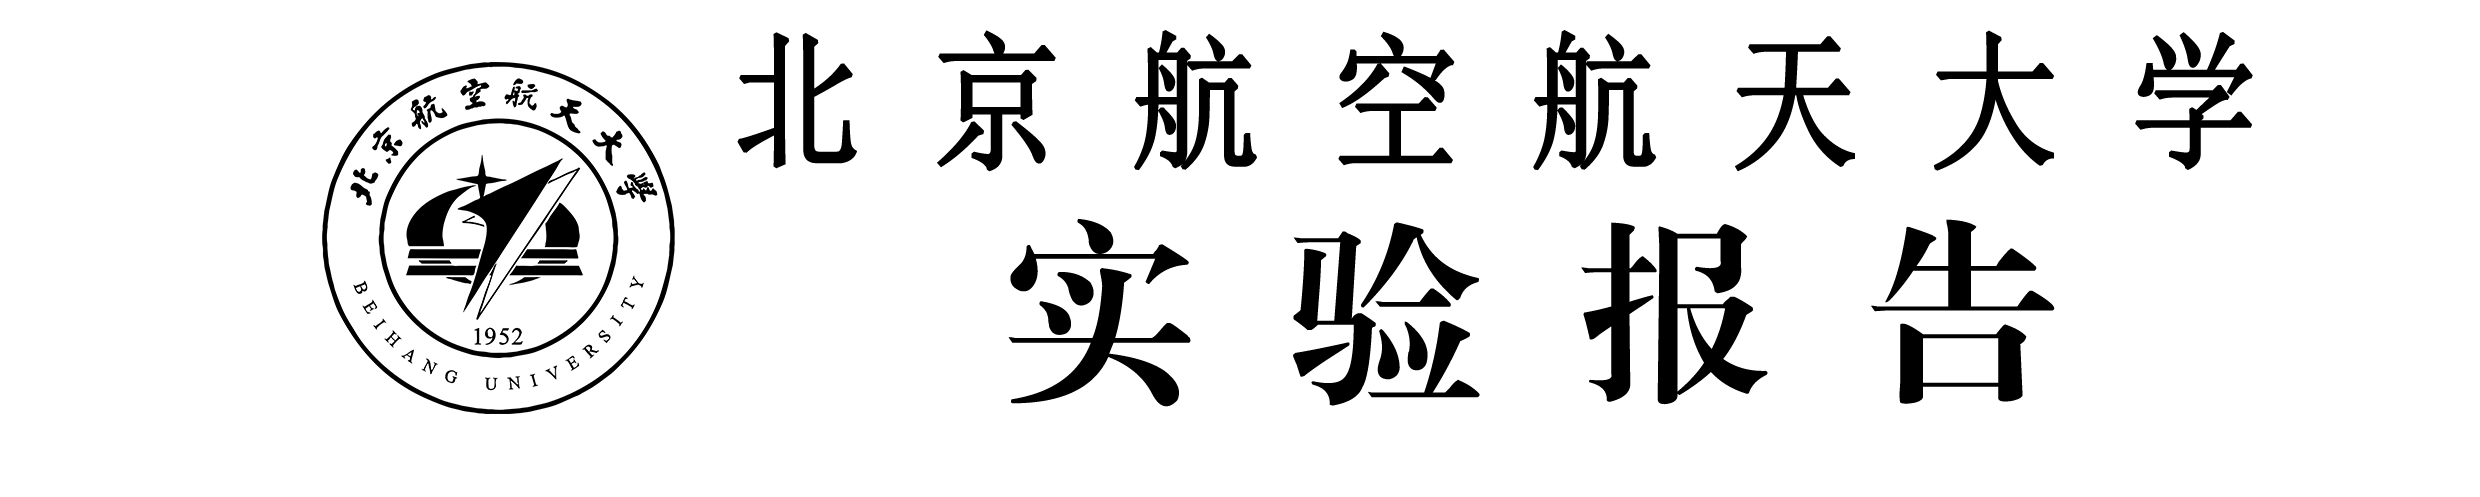
\includegraphics[width=13cm]{表头.png}
\end{figure}
\begin{center}
\textbf{{\large 实验名称:\uline{          测定水的溶解热及电热法测量焦耳热的当量       }}}
\end{center}

\section*{一、实验目的}
\begin{enumerate}
\item 熟悉热学实验中的基本问题——量热和计温;
\item 研究电热法中作功与传热的关系;
\item 学习两种进行散热修正的方法——牛顿冷却定律法和一元线性回归法;
\item 了解热学实验中合理安排实验和选择参量的重要性;
\item 熟悉热学实验中基本仪器的使用。
\end{enumerate}

\section*{二、 实验原理}
\subsection*{1.测量冰的熔解热实验}
	若有质量为M,温度为${T_1}$的冰(在实验室环境下其比热容为$c_1$,熔点为$T_0$),与质量为m,温度为$T_2$的水(比热容为$c_0$)混合,冰全部溶解为水后的平衡温度为$T_3$,设量热器的内筒和搅拌器的质量分别为$m_1$、$m_2$,比热容分别为$c_1$、$c_2$,温度计的热容为${\delta}_m$。如果实验系统为孤立系统,将冰投入盛水的量热器中,则热平衡方程式为
\begin{center}
$c_{1}M(T_{0}-T_{1})+ML+c_{0}M(T_{3}-T_{0})=(c_{0}m+c_{1}m_{1}+c_{2}m_{2}+\delta m)(T_{2}-T_{3})     (1)$
\end{center}
式中,L为冰的熔解热。

在本实验条件下,冰的熔点也可认为是0℃,即$T_0$=0℃,所以冰的熔解热为
\begin{center}
	$L=\frac{1}{M}(c_{0}m+c_{1}m_{1}+c_{2}m_{2}+\delta m)(T_{2}-T_{3})-c_{0}T_{3}+c_{1}T_{1}
	     (2)$
\end{center}

  在作精密测量时,就需要采用一些办法来求出实验过程中实验系统究竟散失或吸收了多少热量,进而对实验结果进行修正。
	一个系统的温度如果高于环境温度它就要散失热量。实验证明,当温度差相当小时(例如不超过10—15℃),散热速率与温度
	差成正比,此即牛顿冷却定律,用数学形式表示可写成
	\begin{center}
	$\displaystyle\frac{\delta q}{\delta t}=K(T-\theta )     (3)$
	\end{center}

  式中,${\delta}_q$是系统散失的热量;是时间间隔;K是散热常数,与系统表面积成正比,并随表面的吸收或发射辐射热的
  本领而变,T、$\theta$分别是所考虑的系统及环境的温度;$\frac{\delta q}{\delta t}$称为散热速率,表示单位时
  间内系统散失的热量。
  
\begin{figure}[H]
 \centering
  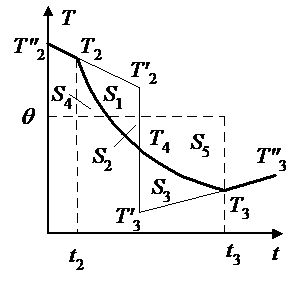
\includegraphics[width=6cm]{系统散热未修正图.png}
\end{figure}

	如图所示,在t=$t_2$时投入冰块,在t=$t_3$时冰块熔化完毕。在投入冰块前,系统的温度沿${T''_2}{T_2}$变化;
	在冰块熔化完毕后,系统温度沿${T_3}{T''_3}$变化。${T''_2}{T_2}$和${T_3}{T''_3}$实际上都很接近
	直线。作${T''_2}{T_2}$的延长线到${T'_2}$,作${T_3}{T''_3}$的延长线到${T'_3}$,连接${T'_2}
	{T'_3}$,使${T'_2}{T'_3}$与T轴平行,且使面积${S_1}+{S_2}={S_3}$,用${T'_2}$代替${T_2}$,用${T'_3}$代替${T_3}$,代入公式(2)求L,就得到系统与环境没有发生热量交换的实验结果。
	
	实际的温度变化本来是${T''_2}{T_2}{T_4}{T_3}{T''_3}$,在冰块投入到冰块熔化完毕的过程中,系统散失的热量相当
	于面积S,从环境吸收的热量相当于面积${S_2}+{S_5}$,综合两者,系统共吸收的热量相当于面积$S={S_2}+{S_5}-{S_4}$。

  在用$T'_2$代替$T_2$、用$T'_3$代替$T_3$后,得到另一条新的温度曲线${T''_2}{T_2}{T'_2}{T'_3}{T_3}
  {T''_3}$。在从冰块投入到冰块熔化完毕的过程中,系统散失的热量相当于面积${S_1}+{S_4}$,从环境吸收的热量相当于      
  面积${S_3}+{S_5}$。综合两者,系统共吸收的热量相当于面积$S'={S_3}+{S_5}-{S_1}-{S_4}$。
	
	因为作图时已使${S_1}+{S_2}={S_3}$,所以有S'=S。这说明,新的温度曲线与实际温度曲线是等价的。

\subsection*{2.电热法测量焦耳热功当量实验}
\subsubsection*{(1)一般说明}
	如图所示,给电阻R两端加上电压V,通过R的电流为I,通电时间t内电场力作功W=VIt。若这些功全部转化为热量,使一个盛水的量热器系统由初温升高至,系统吸收的热量为Q,则热功当量J=W/Q。按照能量守恒定律,若采用国际单位制,则W和Q的单位都是焦耳(J),比值J=1;若Q用卡(cal)作单位,则J=4.1868 J/cal,表示产生1卡热量所需作的功。
	
	实验在装水的量热筒中进行。系统吸收的热量为
\begin{center}
$Q=(c_{0}m_{0}+c_{1}m_{1}+c_{2}m_{2})(\theta -\theta_{0})=Cm(\theta-\theta_{0})     (4)$
\end{center}

式中, $c_0$、$c_1$、$c_2$ 分别是水、量热装置及加热器的比热容;$m_0$、$m_1$、$m_2$分别是其相对应的质量;${C_m}={c_0}{m_0}+{c_1}{m_1}+{c_2}{m_2}$是系统的总热容;${\theta}_0$为系统初温。本实验的主要内容就是测定热功当量$J=VIt/Cm(\theta-\theta_{0})$。
\subsubsection*{(2)散热修正}

\begin{wrapfigure}{r}{0.4\textwidth}
  \vspace{-20pt}
  \begin{center}
    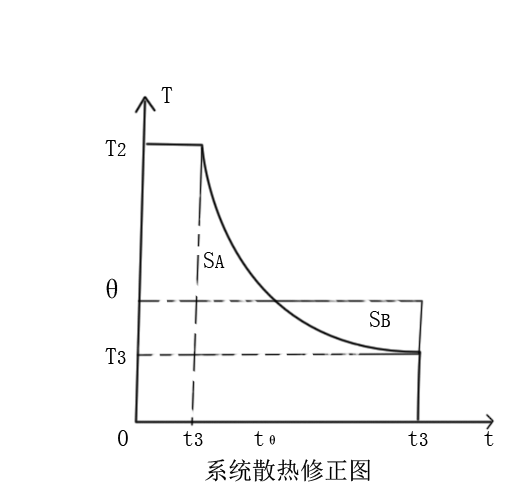
\includegraphics[width=0.48\textwidth]{系统散热修正图.png}
  \end{center}
  \vspace{-20pt}
  \vspace{-10pt}
\end{wrapfigure}

	本实验的难点是如何考虑系统散热的修正。我们从系统应满足的微分方程出发。若把系统看成是理想绝热的,即只考虑系统由于通电而升温,则由系统吸热方程$Q=Cm(\theta-{\theta}_0)$对时间求导可以得到温度变化率所满足的关系式为\\
\begin{center}
$\displaystyle\frac{d\theta}{dt} |_{\text{吸}}=\displaystyle\frac{VI}{JCm}     (5)$
\end{center}
	考虑通电时系统吸热的同时也向环境中放热,根据牛顿冷却定律,由于放热引起的温度变化率为
	\begin{center}
$\displaystyle\frac{d\theta}{dt} |_{\text{放}}=-K(\theta-\theta_{\text{环}})     (6)$
	\end{center}

式中,K为系统的散热系数。综合式(5)和式(6)描述的吸热、放热效应,系统温度的实际变化率为
\begin{center}
$\displaystyle\frac{d\theta}{dt}=\displaystyle\frac{VI}{JCm}-K(\theta - \theta_{\text{环}})    (7)$
\end{center}
这是一个一阶线性的常系数微分方程。我们试图利用一元线性回归法处理数据,令$y=\frac{d\theta}{dt}$,$x=\theta-\theta_{\text{环}} $,式(7)变成y=a+bx,其中$a=\frac{VI}{JCm}$,b=-K。给加热系统通电,并同时记录系统温度—时间的变化关系,每隔1min记录一次温度,共测30个连续时间对应的温度值,即
($t_1$,${\theta}_1$),($t_2$,${\theta}_2$),…($t_30$,${\theta}_30$),这样由一系列($t_i$,$\theta_i$)就换算出($y_i$,$x_i$)数据了,代入回归系数计算式求得a,从而由下式计算出热功当量J(式中R是加热用的电阻值),即
\begin{center}
$a=\displaystyle\frac{v^{2}}{RJCm}\rightarrow J=\displaystyle\frac{v^{2}}{aRCm}     (8)$
\end{center}

\section*{三、 实验仪器}
量热器、电子天平、温度计、数字三用表、加血器皿、冰、水桶、停表、干拭布等。

\section*{四、 实验步骤}
\subsection*{实验1.测量冰的熔解热实验}
\subsubsection*{(1)测定冰的熔解热实验}
一个成功的实验应能测量出投冰前的降温曲线和冰块熔化后的升温曲线,且系统终温T低于环境温度(温度差不超过15℃)。影响实验结果的参量有水的质量m、水的初温T以及冰的质量M,而这些参量的大小是互相制约的,需要先定出它们的取值范围,再通过实验进行调整。
	
首先,冰块的大小是基本固定的,可根据量热筒的大小选择投放一块或两块冰。

其次,确定水的初温T。一般选择T高于环境温度10—15℃,因为此时的散热服从牛顿冷却定律,便于对系统散热进行粗略修正。

最后,当M与T确定后,要想调整实验结果,只有通过改变水的质量m来实现了。水的质量不宜太大,水多需要的冰块就多,否则测不出升温曲线;水也不能太少,太少不利于搅拌,且会使系统终温T过低。可取量热筒内筒的1/2—1/3进行试探性实验,如果未能测出升温曲线,或最终T低于室温15℃以上,则需要改变水量重新做实验。
\subsubsection*{(2)记录有关常数}
称量各种质量。注意冰不能直接放在天平盘上称量,冰的质量应由冰溶解后,冰加水的质量减去水的质量求得。
\subsubsection*{(3)测定实验过程中系统温度随时间的变化}
i).每隔一定时间测系统温度,作T—t图。\\
ii).实测系统的散热温度K——量热器盛适量水,水温比环境温度低5—10℃,测量系统温度随时间的变化。
\subsubsection*{(4)数据处理}
i).用第二种散热修正方法,作图求出初、末温度的修正值,并算出冰的熔解热L。\\
ii).由测量数据估算系统的散热常数K。

\subsection*{实验2.电热法测量焦耳热功当量实验}
\begin{enumerate}
\item  称量各种质量\\
提示:水的质量不宜过大或过小,一般控制在200—240g为好。加热器由功率电阻组成,搅拌器主要由铝制叶片组成,两者的总热容可按64.35 J/ K计算。
\item  测量时间—温度关系\\
 在连续升温的30min内,应等间隔地读取31个温度值(每分钟1次)。
\item  测量加热器的电功率\\
分别在读数始末,用数字三用表测出加热器两端的电压(注意三用表的插孔位置和量程选择)
\item  数据处理\\
用一元线性回归方法计算热功当量J并与理论值对比,计算它们的相对误差。
\end{enumerate}

\end{document}